\documentclass{exam}

\usepackage{units} 
\usepackage{graphicx}
\usepackage[fleqn]{amsmath}
\usepackage{cancel}
\usepackage{float}
\usepackage{mdwlist}
\usepackage{booktabs}
\usepackage{cancel}
\usepackage{polynom}
\usepackage{caption}
\usepackage{fullpage}
\usepackage{xfrac}
\usepackage{enumerate}

\newcommand{\degree}{\ensuremath{^\circ}} 
\everymath{\displaystyle}

\printanswers

% \begin{figure}[H]
%   \centering
%   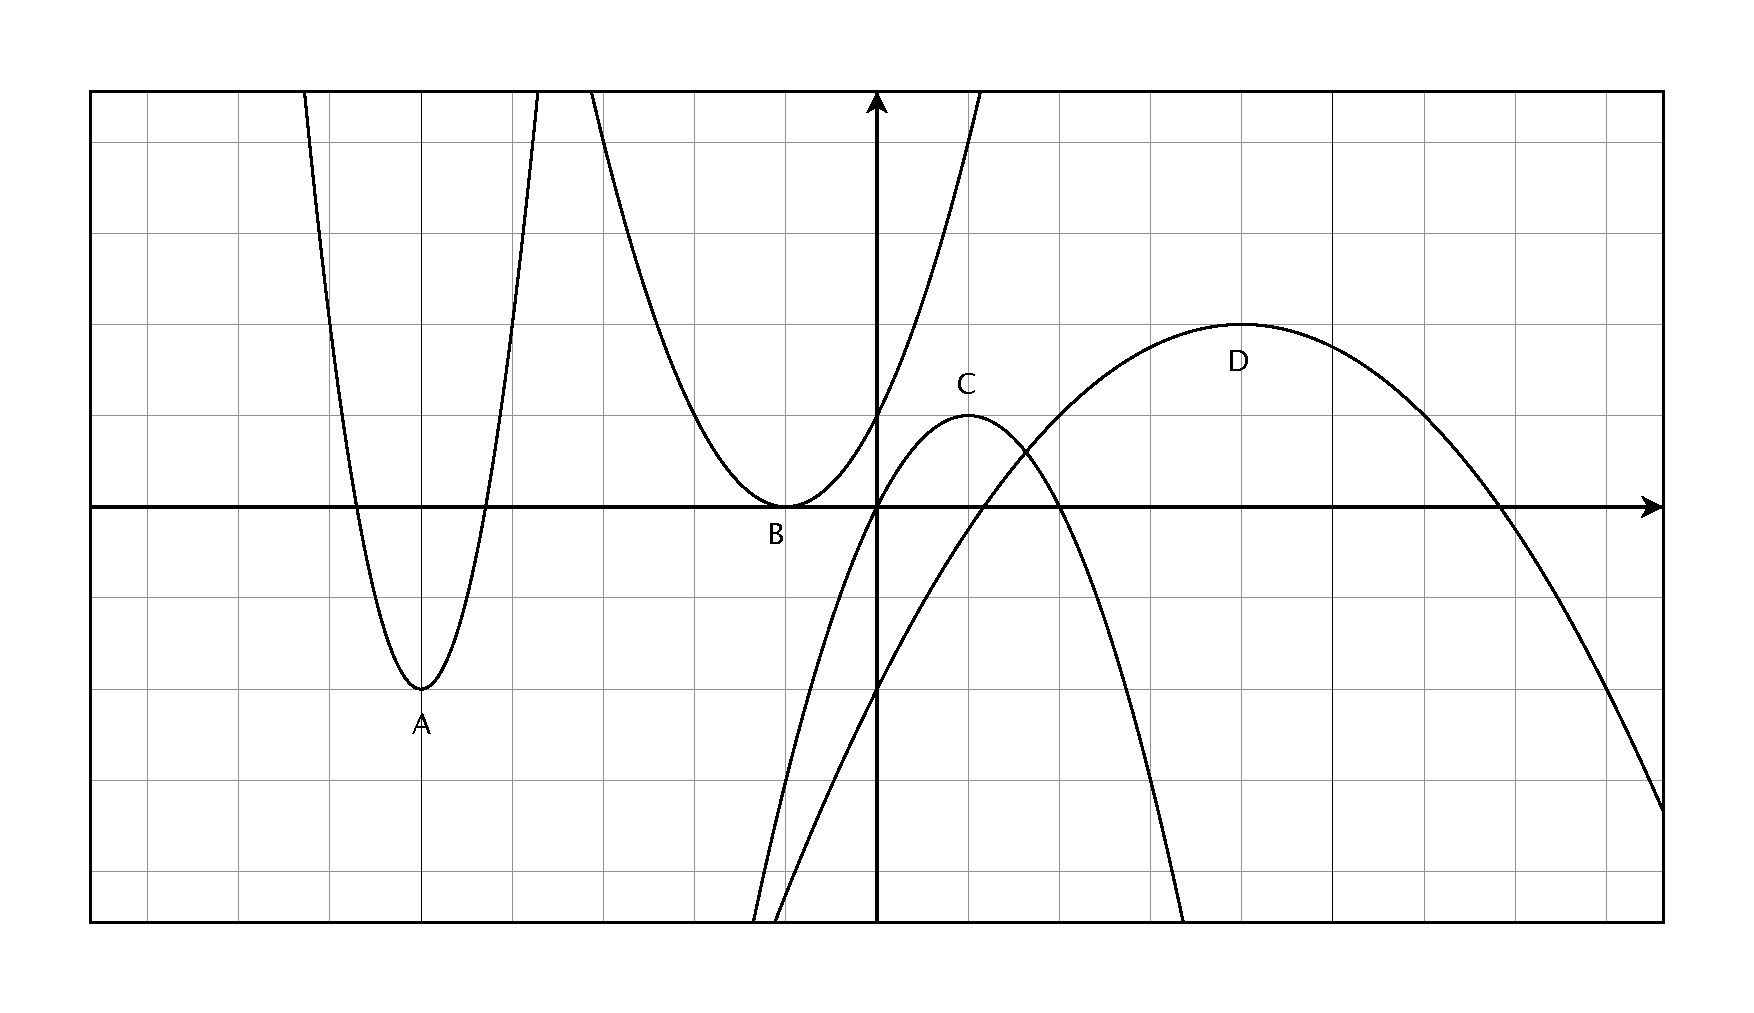
\includegraphics[scale=.3]{problem_7.eps}
%   \caption*{Problem 7}
% \end{figure}

% \begin{tabular}{cc}
% \toprule
% period & amplitude \\
% \midrule
%   $\pi$ & $2$ \\
% \bottomrule
% \end{tabular}

\title{Math 141 Notes \\ Section 3.2}
\date{April 3, 2013}

\begin{document}

  \maketitle
  \tableofcontents

  \section{Long Division}
  \subsection{Description}

  \begin{itemize*}
    \item Show sample dividing decimals
    \item Show dividing polynomials is similar
  \end{itemize*}

  Ways of writing expressing division:

  \begin{align*}
    \frac{P(x)}{D(x)} &= Q(x) + \frac{R(x)}{D(x)} \\
    P(x)              &= D(x) \cdot Q(x) + R(x) \\
  \end{align*}

  \subsection{Examples}

  \begin{enumerate}

    \item 
      \[ \frac{x^2 - 3x + 2}{x - 4} = (x + 1) + \frac{6}{x - 4} \]

      \[ \polylongdiv{x^2 - 3x + 2}{x - 4} \]

    \item 
      \[ \frac{2x^3 + 3x + 2}{x - 2} = (2x^2 + 4x + 11) + \frac{24}{x - 2} \]
      \[ \polylongdiv{2x^3 + 3x + 2}{x - 2} \]

    \item 
      \[ \frac{4x^2 + 3x + 5}{2x + 1} = \left( 2x + \frac{1}{2} \right) + \frac{9}{2(2x + 1)} \]
      \[ \polylongdiv{4x^2 + 3x + 5}{2x + 1} \]

    \pagebreak

    \item 
      \[ \frac{6x^5 + 4x^4 + x^3 + 10x^2 + 2x + 6}{2x^2 + 1} = 3x^3 + 2x^2 - x + 4 + \frac{3x + 2}{2x^2 + 1} \]

      \[ \polylongdiv{6x^5 + 4x^4 + x^3 + 10x^2 + 2x + 6}{2x^2 + 1} \]

  \end{enumerate}

  \section{Synthetic Division}

  \subsection{Description}

  Shortcut when dividing by $x - c$

  \[ \frac{2x^4 - 5x^3 + 5x^2 + x - 9}{x - 2} = (2x^3 - x^2 + 3x + 7) + \frac{5}{x - 2} \]

  \[ \polylongdiv{2x^4 - 5x^3 + 5x^2 + x - 9}{x - 2} \]

  \[ \polyhornerscheme[x = 2]{2x^4 - 5x^3 + 5x^2 + x - 9} \]

  \pagebreak

  \subsection{Examples}
  \begin{enumerate}
    \item 
      \[ \frac{4x^2 - 7x - 21}{x - 4} = (4x + 9) + \frac{15}{x - 4} \]
      \[ \polyhornerscheme[x = 4]{4x^2 - 7x - 21} \]

    \item 
      \[ \frac{3x^3 + 5x^2 - 7x + 2}{x + 1} = (3x^2 + 2x - 9) + \frac{11}{x + 1} \]
      \[ \polyhornerscheme[x = -1]{3x^3 + 5x^2 - 7x + 2} \]
      
    \item 
      \[ \frac{4x^3 + x - 1}{x - 1} = (4x^2 + 4x + 5) + \frac{4}{x - 1} \]
      \[ \polyhornerscheme[x = 1]{4x^3 + x - 1} \]
      
    \item 
      \[ \frac{2x^4 + x^3 - 2x^2 - 11x + 4}{x + 2} = (2 x^3-3 x^2+4 x-19) + \frac{42}{x + 2} \]
      \[ \polyhornerscheme[x = -2]{2 x^4 + x^3 - 2 x^2 - 11x + 4} \]

  \end{enumerate}

  \section{Remainder Theorem}
  \subsection{Description}

  Remainder of $\frac{P(x)}{x - c}$ is $P(c)$.

  Proof:
  \begin{align*}
    \frac{P(x)}{x - c} &= Q(x) + \frac{r}{x - c} \\
    P(x)               &= Q(x) (x - c) + r \\
    P(c)               &= Q(x) (c - c) + r \\
                       &= r \\
  \end{align*}

  \subsection{Examples}
  \begin{enumerate}

    \item 
      \begin{align*}
        P(x) = x^3 + 5 x^2 - 8 x + 1 \\
        P(2) &= 13 \\
      \end{align*}

      \[ \polyhornerscheme[x = 2]{x^3 + 5 x^2 - 8 x + 1} \]

    \item 
      \begin{align*}
        P(x) &= x^4 - 3 x^3 - 8 x^2 + 2 x + 3 \\
        P(5) &= 63 \\
      \end{align*}

      \[ \polyhornerscheme[x = 5]{x^4 - 3x^3 - 8x^2 + 2x + 3} \]

  \end{enumerate}

  \section{Factor Theorem}

  \subsection{Description}

  $c$ is a zero of $P$ if and only if $(x - c)$ is a factor of $P$.

  Proof:

  If $(x - c)$ is a factor of $P(x)$:
  \begin{align*}
    P(x) &= Q(x)(x - c) \\
    P(c) &= Q(c)(c - c) \\
         &= 0 \\
  \end{align*}

  If $P(c) = 0$, then from the {\em Remainder Theorem}:
  \begin{align*}
    P(x) &= Q(x)(x - c) + 0 \\
         &= Q(x)(x - c) \\
  \end{align*}

  \subsection{Examples}
  \begin{enumerate}

    \item 
      \begin{align*}
        P(x) &= x^3 + x^2 - 10x + 8 \\
             &= (x + 4)(x - 1)(x - 2) \\
      \end{align*}

      \[ \polyhornerscheme[x = -4]{x^3 + x^2 - 10x + 8} \]

    \item 
      \begin{align*}
        P(x) &= x^3 - x^2 - 41x + 105 \\
             &= (x + 7)(x - 5)(x - 3) \\
      \end{align*}

      \[ \polyhornerscheme[x = 5]{x^3 - x^2 - 41x + 105} \]

      or

      \[ \polyhornerscheme[x = -7]{x^3 - x^2 - 41x + 105} \]

      or

      \[ \polyhornerscheme[x = 3]{x^3 - x^2 - 41x + 105} \]

  \end{enumerate}

  \pagebreak

  \section{Finding Polynomials with Specified Zeros}

  \begin{enumerate}
    \item Find a polynomial of degree 3 with zeros at $-3$, $2$, and $4$.
      \[
        P(x) = (x + 3)(x - 2)(x - 4) = x^3 - 3x^2 - 10x + 24
      \]
      
      \begin{figure}[H]
        \centering
        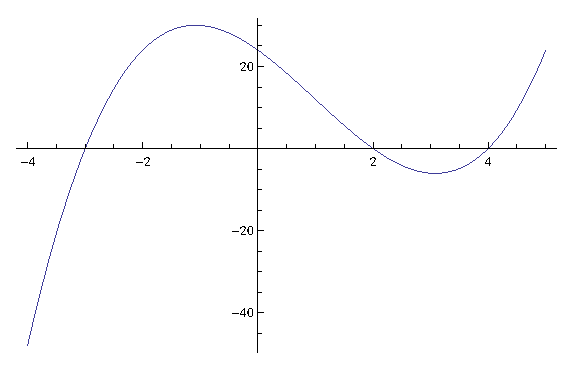
\includegraphics[scale=0.9]{graph1.eps}
        \caption*{$P(x) = x^3 - 3x^2 - 10x + 24$}
      \end{figure}

    \item Find a polynomial of degree 5 with zeros at $-1$ and $2$.  There are multiple possibilities.
      \begin{align*}
        f(x) &= (x + 1)^3(x - 2)^2 \\
        g(x) &= (x + 1)(x - 2)^4 \\
      \end{align*}
      
      \begin{figure}[H]
        \centering
        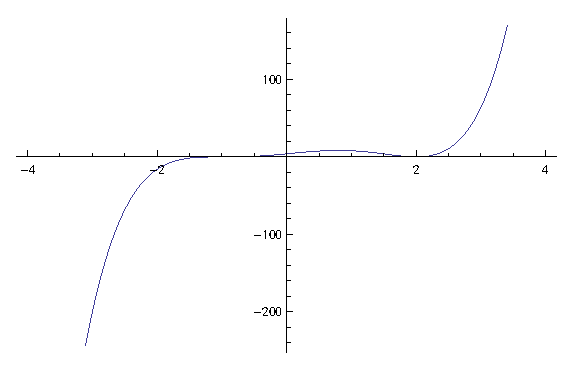
\includegraphics[scale=0.9]{graph2.eps}
        \caption*{$P(x) = (x + 1)^3(x - 2)^2$}
      \end{figure}

      \begin{figure}[H]
        \centering
        
\includegraphics[scale=0.9]{graph3.eps}
        \caption*{$P(x) = (x + 1)(x - 2)^4$}
      \end{figure}
  \end{enumerate}

\end{document}
